\documentclass{article}
\usepackage[utf8x]{inputenc}
\usepackage{ucs}
\usepackage{amsmath} 
\usepackage{amsfonts}
\usepackage{upgreek}
\usepackage[english,russian]{babel}
\usepackage{graphicx}
\usepackage{float}
\usepackage{textcomp}
\usepackage{hyperref}
\usepackage{geometry}
  \geometry{left=2cm}
  \geometry{right=1.5cm}
  \geometry{top=1cm}
  \geometry{bottom=2cm}
\usepackage{tikz}
\usepackage{ccaption}
\usepackage{multicol}

\usepackage{listings}
%\setlength{\columnsep}{1.5cm}
%\setlength{\columnseprule}{0.2pt}


\begin{document}
\pagenumbering{gobble}

\lstset{
  language=C++,                % choose the language of the code
  basicstyle=\linespread{1.1}\ttfamily,
  columns=fixed,
  fontadjust=true,
  basewidth=0.5em,
  keywordstyle=\color{blue}\bfseries,
  commentstyle=\color{gray},
  stringstyle=\ttfamily\color{orange!50!black},
  showstringspaces=false,
  %numbers=false,                   % where to put the line-numbers
  numbersep=5pt,
  numberstyle=\tiny\color{black},
  numberfirstline=true,
  stepnumber=1,                   % the step between two line-numbers.        
  numbersep=10pt,                  % how far the line-numbers are from the code
  backgroundcolor=\color{white},  % choose the background color. You must add \usepackage{color}
  showstringspaces=false,         % underline spaces within strings
  captionpos=b,                   % sets the caption-position to bottom
  breaklines=true,                % sets automatic line breaking
  breakatwhitespace=true,         % sets if automatic breaks should only happen at whitespace
  xleftmargin=.2in,
  extendedchars=\true,
  keepspaces = true,
}
\lstset{literate=%
   *{0}{{{\color{red!20!violet}0}}}1
    {1}{{{\color{red!20!violet}1}}}1
    {2}{{{\color{red!20!violet}2}}}1
    {3}{{{\color{red!20!violet}3}}}1
    {4}{{{\color{red!20!violet}4}}}1
    {5}{{{\color{red!20!violet}5}}}1
    {6}{{{\color{red!20!violet}6}}}1
    {7}{{{\color{red!20!violet}7}}}1
    {8}{{{\color{red!20!violet}8}}}1
    {9}{{{\color{red!20!violet}9}}}1
}


\title{Семинар \#8: Библиотека SFML. Событийно-ориентированное программирование. Классные задачи.\vspace{-5ex}}\date{}\maketitle
\section*{Часть 1: Основные типы и классы библиотеки SFML}
\subsubsection*{Типы целых чисел}
Так как библиотека SFML кросплатформенная, то в ней введены \texttt{typedef}-синонимы для целочисленных типов, например \texttt{Int8}, \texttt{Int64}, \texttt{Uint32} и другие. Эти типы гарантируют, что они будут соответствующего размера.

\subsubsection*{Классы математических векторов}
Классы двумерных математических векторов \texttt{sf::Vector2<T>}. У них есть два публичных поля: \texttt{x} и \texttt{y}. Также, для них перегруженны операции сложения с такими же векторами и умножения на числа. Также введены \texttt{typedef}-синонимы вроде \texttt{sf::Vector2f} для \texttt{sf::Vector2<float>} и другие.

\subsubsection*{Класс цвета}
Класс цвета \texttt{sf::Color}. Имеет 4 публичных поля: \texttt{r}, \texttt{g}, \texttt{b}, \texttt{a} - компоненты цвета в цветовой модели RGB и прозрачность. Есть конструктор от 3-х или 4-х аргументов. Есть перегруженные операции для сравнения и сложения цветов. Есть уже определённые цвета вроде \texttt{sf::Color::Blue} и другие.

\subsubsection*{Класс строки}
В SFML есть свой класс строки под названием \texttt{sf::String}. Поддерживает разные виды кодировок. Имеет конструкторы от стандартных строк \texttt{C++} и строк в стиле \texttt{C}.

\subsubsection*{Класс окна}
Прежде чем начать рисовать, нужно создать окно, которое будет отображать то, что мы нарисовали. Для этого в SFML есть класс \texttt{sf::RenderWindow}. Вот его основные методы:
\begin{itemize}
\item \texttt{RenderWindow(sf::VideoMode m, const sf::String\& title, sf::Uint32 style, sf::ContextSettings\& s)}
Конструктрор, с двумя обязательными и двумя необязательными аргументами. Его аргументы:
\begin{itemize}
\item Видеорежим - определяет размер окна.
\item Заголовок окна
\item Стиль окна, необязательный аргумент, может принимать следующие значения:
\begin{itemize}
\item[-] \texttt{sf::Style::None}
\item[-] \texttt{sf::Style::Titlebar} -- окно с заголовком
\item[-] \texttt{sf::Style::Resize}  -- окно у которого можно менять размер
\item[-] \texttt{sf::Style::Close} -- окно с кнопочкой закрывания
\item[-] \texttt{sf::Style::Fullscreen} -- полноэкранный режим
\item[-] \texttt{sf::Style::Default = sf::Titlebar | sf::Resize | sf::Close} 
\end{itemize}
Этот параметр имеет значение по умолчанию (\texttt{sf::Default}).

\item Дополнительные настройки контекста OpenGL, необязательный аргумент.
\end{itemize}

\item \texttt{getPosition} и \texttt{setPosition} - получить или установить положение окна.
\item \texttt{getSize} и \texttt{setSize} - получить или установить размер окна в пикселях.
\item \texttt{setFramerateLimit} -- установить лимит для количества кадров в секунду.
\item \texttt{clear} - принимает цвет и очищает скрытый холст этим цветом
\item \texttt{draw} - рисует объект на скрытый холст
\item \texttt{display} - отображает на экран всё что было нарисовано на скрытом холсте
\end{itemize}


\subsubsection*{Классы фигур}
В SFML есть несколько классов для работы с простыми фигурами: \texttt{sf::CircleShape} (круг или элипс),\\ \texttt{sf::RectangleShape} (прямоугольник), \texttt{sf::ConvexShape} (фигура сложной формы, задаваемая точками). У этих классов есть общие методы:
\begin{itemize}
\item \texttt{setOrigin} - установить локальное начало координат фигуры. Положение этой точки задаётся относительно верхнего левого угла прямоугольника, ограничивающего фигуру. По умолчанию эта точка равна \texttt{(0, 0)}, то есть локальным началом координат фигуры считается её верхний левый угол.  Эта точка важна, так как относительно неё происходят все операции поворота и масштабирования.
\item \texttt{setPosition}, \texttt{getPosition} - задать и получить координаты фигуры. Фигура перемещается таким образом, чтобы её \texttt{origin} оказался в заданой точке.
\item \texttt{move} - принимает 2D вектор и передвигает фигуру на этот вектор.
\item \texttt{setRotation}, \texttt{getRotation} - задать и получить угол (в градусах) вращения фигуры вокруг точки \texttt{origin}
\item \texttt{rotate} - принимает вещественное число и вращает фигуру на этот угол (в градусах)
\item \texttt{setScale}, \texttt{getScale} - задать и получить величину масштабирования (2D вектор)
\item \texttt{scale} - принимает  2D вектор и растягивает или сжимает фигуру по x и по y соответственно
\item \texttt{setFillColor}, \texttt{getFillColor} -- устанавливает/возвращает цвет заливки фигуры
\end{itemize}

\subsubsection*{Задачи:}
\begin{itemize}
\item В папке \texttt{00circle} приведён пример программы, которая рисует круг. Измените эту программу, чтобы круг рисовался в левом верхнем углу экрана.
\item Измените эту программу, чтобы круг рисовался в правом нижнем углу экрана.
\item Нарисуйте 100 кругов в случайных местах экрана, случайного размера и случайного цвета.
\item В папке \texttt{01shapes} приведён пример программы, которая рисует несколько фигур. Используйте методы выше и сделайте так, чтобы круг двигался по прямой, прямоугольник вращался, а фигура сложной формы сжималась по y и растягивалась по x. Подберите скорости этих операций, чтобы они были не слишком быстрыми.
\item Перейдите в полноэкранный режим
\end{itemize}

\subsubsection*{Anti-Aliasing}
\begin{multicols}{2}
\begin{center}
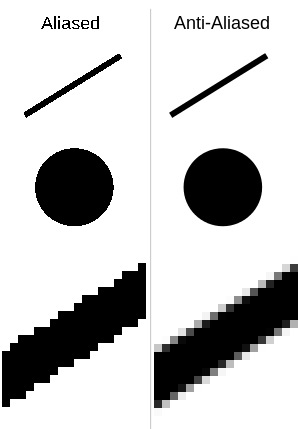
\includegraphics[scale=0.5]{../images/anti-aliasing.png}
\end{center}
Вы могли заметить, что фигуры выглядят не очень красиво - имеют зазубрены. Это связано с тем, что рисования происходит на прямоугольной сетке пикселей и при проведении линий под углом образуются ступеньки. Для борьбы с этим эффектом был придуман специальный метод сглаживания, который называется антиалиасинг. Он уже автоматически реализован во всех библиотеках компьютерной графики. Чтобы установить его в SFML, нужно прописать опцию:
\begin{lstlisting}
sf::ContextSettings settings;
settings.antialiasingLevel = 8;
\end{lstlisting}
И передать \texttt{settings} на вход для конструктора \texttt{RenderWindow}. Пример в папке \texttt{02antialiasing}.
\end{multicols}

\newpage
\subsection*{Главный цикл}
Как правило, у любой программы, работающей на основе событийно-ориентированной модели, есть главный цикл. На каждой итерации данного цикла программа должна проделать все необходимые операции по подготовке и отрисовке следующего кадра. Число итераций этого цикла называется числом кадров в секунду (англ. frames per seconds - fps).

В папке \texttt{4mainloop} предсталена простейшая программа с главным циклом. Сейчас основной цикл программы работает без перерывов и, так как наша программа очень проста, то количество кадров в секунду может достигать огромных значений - больше 1000 fps. Мониторы не обновляют экран с такой скоростью и человеческий глаз тоже не способен воспринять такую частоту кадров. Поэтому не имеет смысла задавать fps очень высоким, его желательно ограничить. Это можно сделать с помощью метода \texttt{setFramerateLimit}. Пример в папке \texttt{06framerate\_limit}.

Этот метод ограничивает лишь максимальное количество кадров. Если за один кадр выполняется много вычислений, то fps может просесть ниже 60. Из за этого программы, которые завязанны на времени, могут работать некорректно. Например, в нашем примере скорость движения шарика зависит от числа кадров в секунду. Чтобы шарик двигался одинаково независимо от fps нужно высчитывать время, занятое на каждом кадре. Пример, как это делать в папке \texttt{07clock\_time}.

\subsubsection*{Класс времени}
Класс \texttt{sf::Time} для работы со временем. Есть методы \texttt{asSeconds}, \texttt{asMilliseconds} и \texttt{asMicroseconds}, которые возвращают время в виде числа в соответствующих единицах. Перегружены операторы сложения, умножения и другие. Есть дружественные функции \texttt{sf::seconds}, \texttt{sf::milliseconds} и \texttt{sf::microseconds}, которые принимают число, и возвращают соответствующие объект класса \texttt{sf::Time}.

\subsubsection*{Класс часов}
\texttt{sf::Clock} -- это маленький класс для измерения времени. У него есть:
\begin{itemize}
\item Конструктор по умолчанию, часы запускаются автоматически после создания.
\item Метод \texttt{getElapsedTime()} -- возвращает объект \texttt{sf::Time} -- время прошедшее с последнего запуска часов.
\item Метод \texttt{restart()} -- заново запускает часы.
\end{itemize}

\subsection*{Проверка на нажатие клавиш и кнопок}
\subsubsection*{Класс клавиатуры}
Класс клавиатуры \texttt{sf::Keyboard}. Внутри этого класса, в публичной части, объявлен перечисляемый тип \texttt{Key}, в котором перечислены все клавиши. Например, чтобы проверить нажатие на пробел понадобится \texttt{sf::Keyboard::Space}. Название всех клавиш можно найти по следующей ссылке: \href{https://www.sfml-dev.org/documentation/2.5.1/classsf_1_1Keyboard.php}{Тут}.\\
У этого класса есть метод 
\begin{itemize}
\item \texttt{isKeyPressed} -- принимает клавишу и проверяет нажата ли она.
\end{itemize}
Пример -- в папке \texttt{08is\_key\_pressed}.


\subsubsection*{Класс мыши}
Класс мыши \texttt{sf::Mouse}. Внутри этого класса, в публичной части, объявлен перечисляемый тип \texttt{Button} в котором перечислены все кнопки мыши.
У этого класса есть метод:
\begin{itemize}
\item \texttt{isButtonPressed} принимает на вход \texttt{sf::Mouse::Button} и проверяет нажата ли соответствующая кнопка.
\item \texttt{getPosition()} -- возвращает положение мыши на в координатах всего экрана.
\item \texttt{setPosition(const sf::Vector2i\&)} --  устанавливает положение мыши на в координатах всего экрана
\item \texttt{getPosition(const sf::Window\&)} -- возвращает положение мыши на в координатах данного окна.
\item \texttt{setPosition(const sf::Vector2i\&, const sf::Window\&)} --  устанавливает положение мыши на в координатах данного окна.
\end{itemize}
Пример -- в папке \texttt{09is\_button\_pressed}.

\subsubsection*{Задачи:}
\begin{itemize}
\item Создайте 2 объекта: круг и квадрат. Круг должен двигаться при нажатии на стрелки. Квадрат должен двигаться при нажатии на \texttt{WASD}.
\item Сделайте так, чтобы при нажатии на левую кнопку мыши координаты круга становились бы равными координатам мыши.
\item Сделайте так, чтобы при нажатии на \texttt{Enter} цвет квадрата менялся случайным образом каждый кадр.
\item Сделайте так, чтобы квадрат передвигался вправо на 50 пикселей каждые 2 секунды. При этом, все остальное должно работать как прежде, то есть функцию \texttt{sf::sleep} использовать не получится.
\item Сделайте так, чтобы цвет круга плавно зависел от положения курсора на экране.

\item Создайте новый круг белого цвета и сделайте так, чтобы при наведении на него курсора, он становился красным.
\end{itemize}


\subsection*{Работа с текстом}
Для работы с текстом есть два класса. Класс шрифта \texttt{sf::Font} и класс текста \texttt{sf::Text}. Пример работы с текстом в папке \texttt{03text}.
\subsubsection*{Задачи:}
\begin{itemize}
\item Создайте вращающийся текст.
\item Сделайте так, чтобы при нажатии клавиши пробел у текста задавалась случайная позиция, случайный поворот, случайный цвет и случайное масштабирование(в разумных пределах).
\item Создайте 2 поля текста. В первом нужно печатать положение мыши в системе отсчёта всего экрана. Во втором поле текста нужно печатать координаты мыши в системе отсчёта окна. Для перевода чисел в строку используйте функцию \texttt{std::to\_string}.
\end{itemize}


\newpage

\section*{Часть 2: События}
\begin{itemize}

\item \textbf{KeyPressed:} В папке \texttt{1key\_events} лежит пример программы, которая обрабатывает нажатия клавиш. Измените программу так, чтобы при нажатии на клавишу Enter кружок менял цвет на случайный.

\item \textbf{KeyReleased:} Измените программу так, чтобы при \textit{отпускании} клавиши пробел прямоугольник менял цвет на случайный (событие \texttt{sf::Event::KeyReleased}).

\item \textbf{MouseButtonPressed:} В папке \texttt{2mouse\_events} лежит пример программы, которая обрабатывает нажатия и движение мыши. Измените программу так, чтобы при нажатии на правую кнопку мыши, прямоугольник перемещался к положению мыши. Событие должно срабатывать только в момент нажатия, прямоугольник не должен двигаться при зажатии кнопки.
\begin{lstlisting}
if (event.type == sf::Event::MouseButtonPressed)
{
    if (event.mouseButton.button == sf::Mouse::Right)
    {
        std::cout << "the right button was pressed" << std::endl;
        std::cout << "mouse x: " << event.mouseButton.x << std::endl;
        std::cout << "mouse y: " << event.mouseButton.y << std::endl;
    }
}
\end{lstlisting}


\item \textbf{MouseMoved:} Событие, которое срабатывает тогда, когда двигается мышь.
\begin{lstlisting}
if (event.type == sf::Event::MouseMoved)
{
    std::cout << "new mouse x: " << event.mouseMove.x << std::endl;
    std::cout << "new mouse y: " << event.mouseMove.y << std::endl;
}
\end{lstlisting}
Измените программу так, чтобы прямоуголиник окрашивался в красный цвет тогда и только тогда, когда курсор мыши находится на прямоугольнике. Во всё остальное время прямоуголиник должен быть зелёным.

\item \textbf{Перетаскивание:} Создайте новый прямоугольник и сделайте его перетаскиваемым. При нажатии на него и последующим движении мыши он должен начать двигаться вместе с курсором. При отпускании мыши должен остаться на месте.



\end{itemize}

\newpage
\section*{Часть 3: Задачи}
\begin{itemize}
\item \textbf{Кнопка:} Создайте "кнопку". Кнопка представляет собой прямоугольник и некий текст поверх этой кнопки. Логика работы должна быть аналогичной логике работы обычной кнопки в ОС Windows. При наведении на прямоугольник он должен немного менять цвет. При зажатии кнопки мыши на прямоугольнике он должен менять цвет на третий. Кнопка должна быть зажата пока зажата кнопка мыши, даже если курсор уже вышел за пределы кнопки. При отпускании мыши, если курсор всё ещё находится на прямоугольнике, должно срабатывать некоторое действие. В качестве действия -- пусть круг будет менять цвет на случайный.

\begin{itemize}
\item Создайте свой класс \texttt{Button}, который будет описывать данное поведение.
\item Используйте этот класс и создайте 4 кнопки с надписями \texttt{Left}, \texttt{Right}, \texttt{Down}, \texttt{Up}. При нажатии на эти кнопки круг должен перемещаться на 20 пикселей в соответствующем направлении. 
\end{itemize}

\item \textbf{Шарики:} В папке \texttt{collision\_circles} содержится заготовка кода. 
\begin{itemize}
\item Используйте этот код, чтобы найти пересечение двух шаров. Если в процессе движения шары начнут накладываются друг на друга, то они должны окрашиваться в красный цвет. После прекращения наложения, шары должны опять стать белыми. Для этого добавьте поле типа \texttt{sf::Color} в класс \texttt{Ball} и метод \texttt{bool is\_colliding(const Ball\& b) const}, который будет проверять 2 кружка на столкновение.
\item Измените программу так, чтобы кружки упруго отскакивали друг от друга. Для этого нужно, при столкновении шариков, обратить составляющую скорости параллельную прямой, соединяющую центры шариков.
\item Добавьте возможность добавления нового шарика по нажатию правой кнопки мыши.
\item Добавьте возможность стенки по нажатию левой кнопки мыши. Нужно зажать ЛКМ в одной точки и отпустить в другой, чтобы получить стенку. Стенка -- это просто отрезок. Но шарики должны от него должны отскакивать. Про обнаружение столкновений можно посмотреть в папке \texttt{collision\_examples}.
\end{itemize}



\item \textbf{Pong:} Создайте игру Pong на 2 игрока. Первый игрок должен управлять ракеткой используя клавиши \texttt{W} и \texttt{S}. Второй игрок -- стрелочки вниз и вверх.
\begin{center}
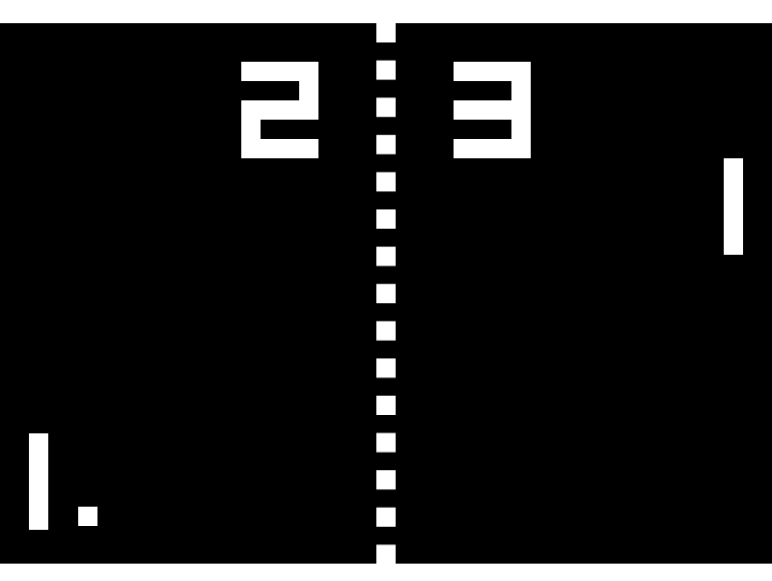
\includegraphics[scale=0.5]{../images/pong.png}
\end{center}
\end{itemize}

\end{document}